\documentclass[12pt]{article}

\usepackage{graphicx,color,enumerate,multicol}
\usepackage[top=1in, bottom=1in, left=1.25in, right=1.25in]{geometry}

%% Use Minion fonts if available.  Otherwise Times.
\IfFileExists{MinionPro.sty}{\usepackage[lf]{MinionPro}}{}
\usepackage{amsmath,amsthm,amsbsy}
\IfFileExists{MinionPro.sty}{}{\usepackage{times,txfonts}}

%% Setup aproblem environment, 
%% aproblem items
%% subproblems environment
%% subproblem items
\makeatletter
\newcounter{probcount}
\newcounter{subprobcount}
\newlength\probsep
\newlength\pshrinking
\newif\iffirstprob
\newenvironment{aproblems}%
  {\ifhmode\unskip\par\fi\setcounter{probcount}{0}\probsep\parskip
  \sbox\@tempboxa{\textbf{9.}}\pshrinking\wd\@tempboxa\advance\pshrinking\labelsep
  \let\hproblem\aproblem
  \advance\linewidth -\pshrinking
  \advance\@totalleftmargin\pshrinking
  \advance\leftskip\pshrinking}%
  {\ifhmode\unskip \par\fi\advance\leftskip-\pshrinking}%

\newcommand{\aproblem}{%
  \setcounter{subprobcount}{0}%
  \stepcounter{probcount}%
  \def\@currentlabel{\arabic{probcount}}%
  \ifhmode
    \unskip \par
  \fi
%  \addpenalty{-4000}%
  \iffirstprob\else\addvspace\probsep\fi
  \firstprobfalse
  \hskip -\labelwidth\hskip -\labelsep 
  \hbox to\labelwidth{\hss\textbf{\arabic{probcount}.}}\hskip\labelsep
}%

\newcommand{\subprob}{\item\def\@currentlabel{\arabic{probcount}\alph{\thelistlabel}}}
\newcommand{\skipproblem}{\stepcounter{probcount}}


%% The following commands put defined left and right headers on the top, and a page number
%% on the bottom of all pages beyond page 1
\usepackage{fancyhdr}
\pagestyle{fancy}
\fancyfoot[C]{\ifnum \value{page} > 1\relax\thepage\fi}
\fancyhead[L]{\ifx\@doclabel\@empty\else\@doclabel\fi}
\fancyhead[R]{\ifx\@docdate\@empty\else\@docdate\fi}
\headheight 15pt
\def\doclabel#1{\gdef\@doclabel{#1}}
\def\docdate#1{\gdef\@docdate{#1}}
\makeatother

%% General formatting parameters
\parindent 0pt
\parskip 6pt plus 1pt

\doclabel{Math F251: Sections 1.1--1.3 Worksheet}
\docdate{16 January 2019}


\begin{document}
\renewcommand{\d}{\displaystyle}

\begin{aproblems}
\aproblem The graph of
a function $f$ is shown below. Find the following:

\begin{quote}
  \begin{multicols}{2}{
      % make sure you added \usepackage{enumerate}
      \vspace*{-0.55in}
      \begin{enumerate}[a)]
      \item $f(1)$ and $f(5)$
      \item the domain of $f$
      \item the range of $f$
      \item For which value of $x$ is $f(x) = 4$?
      \item Where is $f$ increasing?
\columnbreak
\begin{center}
  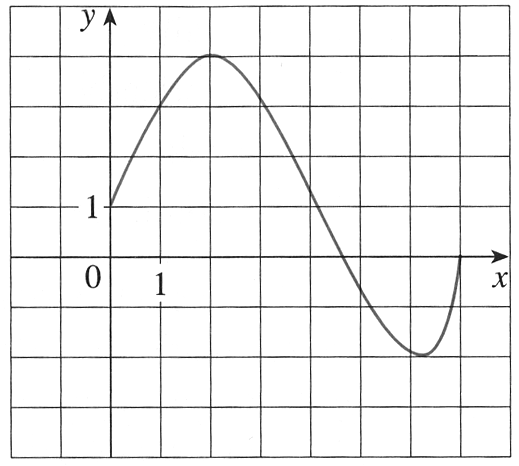
\includegraphics[width=2.8in]{1-1-fig-6}
\end{center}
      \end{enumerate}}
\end{multicols}
\end{quote}

\aproblem  Let $f(x) = 3x^2 - x + 2.$ Find and simplify the following expressions.

% \begin{quote}
  % \begin{multicols}{2}{
      % make sure you added \usepackage{enumerate}
      % \vspace*{-0.45in}
      \begin{enumerate}[(a)]
      \item $f(2)$\vskip 1cm

      \item $f(a^2)$\vskip 1cm

      \item $[f(a)]^2$\vskip 1cm

      \item $\d \frac{f(2+h) - f(2)}{h}$\vskip 1in

      \item $\d \frac{f(a+h) - f(a)}{h}$\vskip 1in
      \end{enumerate}
      % }
  % \end{multicols}
% % \end{quote}
% \vspace{.3in}
% \aproblem Write a formula for the top half of the circle with center $(2,0)$ and radius 3.

\newpage
\aproblem Find the domain of each of the following functions. Use interval notation.
\begin{enumerate}
\item $f(x) = \d \frac{1}{x^4 - 16}$
\vfill
      \item  $f(x) = \sqrt{x} + \sqrt{11 - x}$
      \vfill
       \item $g(x) = \ln( x - 4 )$
       \vfill
      \item $h(x) = \frac{1}{\sqrt{x^2 - 5x - 6}}$
      \vfill
\end{enumerate}

\aproblem Graph each of the following piecewise defined functions.
\begin{multicols}{2}{
      \vspace*{-0.45in}
      \begin{enumerate}[a)]
      \item $f(x) =
        \begin{cases}
          -1\; &\text{if} \; x \ge 2 \\
          7 - 2x \; & \text{if} \; x < 2
        \end{cases}$
        
         \item $f(x) =
        \begin{cases}
          x+1 \; &\text{if} \; x \le - 1 \\
          x^2 \; &\text{if} \; x > -1
        \end{cases}$
\end{enumerate}}
  \end{multicols}
  \vspace{2in}
\end{aproblems}
\end{document}
